\section{Modellierung des Antriebsstranges} \label{modellierung_antriebsstrang}
% Aaron

Dieser Abschnitt befasst sich mit der Modellierung und Simulation des Antriebsstranges der Windturbine. Das Modell soll anschließend zusammen mit dem Modell des Turmes und des Blattes, sowie der Aerodynamik als Teilmodelle in Simulink zusammengeführt werden. \\
Der Antriebsstrang besteht dabei grundsätzlich aus einem Rotor (Blätter und Nabe), einem Getriebe, einem Synchrongenerator sowie einer Welle, welche alle Komponenten mechanisch verbindet. \autoref{fig:Bild3.1} zeigt einer Übersichtsgrafik der Modellparameter als Ein- \bzw Ausgänge des Teilmodells.

\begin{figure}[H]
   \centering
   \begin{pspicture}[showgrid=false](0,0)(10,5)
        \psframe(0,0)(10,5)
        % Eingänge
        \psline{->}(1,3.5)(3.5,3.5)
        \rput(1,3.9){\footnotesize \acs{MG}}
        \psline{->}(1,2.5)(3.5,2.5)
        \rput(1,2.9){\footnotesize \acs{MR}}
        % Modell
        \psframe[linecolor=black,fillcolor=lightGrey,fillstyle=solid](3.5,0.5)(6.5,4.5)
        \rput(5,3.5){\small Modell des}
        \rput(5,3){\small Antriebsstranges}
        % Ausgänge
        \psline{->}(6.5,3.5)(9,3.5)
        \rput(9,3.9){\footnotesize \acs{omegaG}}
        \psline{->}(6.5,2.5)(9,2.5)
        \rput(9,2.9){\footnotesize \acs{omegaR}}
    \end{pspicture}
   \caption[Übersicht Antriebsstrangteilmodell]{Blockdarstellung des Antriebsstrangteilmodells inklusive der Ein- und Ausgangsparameter}
   \label{fig:Bild3.1}
\end{figure} % Teilmodell Antriebsstrang mit Ein- und Ausgangsparametern

Zu erkennen sind das \ac{MG} und das \ac{MR} als Eingangsgrößen des Modells. Das \acl{MR} wird in der Gesamtsimulation später vom Modell der Aerodynamik bereitgestellt. Das \acl{MG} geht aus dem Generator-Umrichter-Modell hervor, in welchem auch die Regelung der Windkraftanlage umgesetzt ist. \\
Als Ausgänge werden die \ac{omegaG} und die \ac{omegaR} benötigt. Erstere ist später ein Eingangsparameter des Generator-Umrichter-Modells und wird insbesondere für die Berechnung des \acl{MG} im Momentenregler benötigt. Die \acl{omegaR} wird für die Berechnung der Stellgröße der beiden Regler für den oberen Teillastbereich und den Volllastbereich zurückgeführt. 

\subsection{Modell des Antriebsstranges}

Zunächst soll das Modell für den Antriebsstrang entwickelt werden, bevor es anschließend simulativ losgelöst in Simulink getestet und verifiziert werden kann. \autoref{fig:Bild3.2} zeigt modellhaft die Struktur des Antriebsstranges mitsamt der wirkenden Momente. Auf Basis der Abbildung erfolgt anschließend die Modellierung des Teilsystems.

\begin{figure}[H]
   \centering
   \begin{pspicture}[showgrid=false](0,0)(14.6,5)
        \psframe(0,0)(14.6,5)
        
        % Generator
        \psline(0.5,2.5)(2.1,2.5)
        \psarc[linecolor=darkgrey]{<-}(2,2.5){1}{150}{210}
        \rput(1.2,3.3){\footnotesize \acs{MG}}
        
        \psellipse(2.1,2.5)(0.3,0.61)
        \psline(2.1,3.1)(3.6,3.1)
        \psline(2.1,1.9)(3.6,1.9)
        \psarc(3.08,2.5){0.8}{-49}{49}
        \rput(3,2.5){\footnotesize \acs{JG}}
        
        \psline(3.9,2.5)(5,2.5)
        \psarc[linecolor=darkgrey]{<-}(3.6,2.5){1}{-30}{30}
        \rput(4.4,3.3){\footnotesize \acs{phiG}}
        
        % Dämpferglied
        \psline(5,3.1)(5,1.9)
        \pscoil[coilwidth=0.3](5,3.1)(7.05,3.1)
        \psline(5,1.9)(5.8,1.9)
        \psline(5.8,2.2)(5.8,1.6)
        \psline(5.8,2.2)(6.5,2.2)
        \psline(5.8,1.6)(6.5,1.6)
        \psline(6,2.15)(6,1.65)
        \psline(6,1.9)(7.05,1.9)
        \psline(7.05,3.1)(7.05,1.9)
        \rput(6,3.7){\footnotesize \acs{ks}}
        \rput(6,1.2){\footnotesize \acs{ds}}
        
        % Getriebe
        \psline(7.05,2.53)(8.1,2.53)
        \psline(7.05,2.47)(8.1,2.47)
        \psarc[linecolor=darkgrey]{<-}(6.7,2.5){1}{-30}{30}
        \rput(7.5,3.3){\footnotesize \acs{phiRtilde}}
        
        \psframe(8.1,1.9)(9.8,3.1)
        \rput(8.9,2.5){\footnotesize \acs{ng}}
        
        % Rotor
        \psline(9.8,2.53)(11.1,2.53)
        \psline(9.8,2.47)(11.1,2.47)
        \psarc[linecolor=darkgrey]{<-}(9.4,2.5){1}{-30}{30}
        \rput(10.2,3.3){\footnotesize \acs{phiR}}
        
        \psellipse(11.1,2.5)(0.3,0.61)
        \psline(11.1,3.1)(12.6,3.1)
        \psline(11.1,1.9)(12.6,1.9)
        \psarc(12.08,2.5){0.8}{-49}{49}
        \rput(11.98,2.5){\footnotesize \acs{JR}}
        
        \psline(12.9,2.5)(14,2.5)
        \psarc[linecolor=darkgrey]{<-}(12.4,2.5){1}{-30}{30}
        \rput(13.2,3.3){\footnotesize \acs{MR}}
    \end{pspicture}
   \caption[Modelldarstellung des Antriebsstranges]{Modellhafte Darstellung des Antriebsstrangteilmodelles inklusive der wirkenden Momente}
   \label{fig:Bild3.2}
\end{figure} % Modelldarstellung des Antriebsstranges inkl. Momente

Die Modellbildung erfolgt über die Momentenbilanzierung. Diese besagt, dass die Summe aller wirkenden Momente gleich Null ist. Zunächst lässt sich die Summe aller Momente allgemein berechnen zu:
\begin{align}
    \sum M = J \cdot \ddot\varphi.
    \label{eq:Gleichung3.1}
\end{align}
\newline
Nachfolgend wird eine Bilanzgleichung für den Generator (high speed shaft) und den Rotor (slow speed shaft) aufgestellt. Erstere ist in \autoref{eq:Gleichung3.2} und Letzere in \autoref{eq:Gleichung3.3} dargestellt.
\begin{align}
    \label{eq:Gleichung3.2}
   \acs{JR} \cdot \ddot{\varphi}_{\mathrm{R}} + \tilde{M}_{d_s} + \tilde{M}_{k_s} - \acs{MR} &= 0 \\
   \label{eq:Gleichung3.3}
   \acs{JG} \cdot \ddot{\varphi}_{\mathrm{G}} - {M}_{d_s} - {M}_{k_s} + \acs{MG} &= 0
\end{align}
\newline
Bei $\tilde{M}_{d_s}$ handelt es sich um das Moment, welches sich aus dem \ac{ds} ergibt. Es wird berechnet zu

\begin{align}
   \tilde{M}_{d_s} = \acs{ds} \cdot \left( \dot\varphi_{\mathrm{G}} - \tilde{\dot\varphi}_{\mathrm{R}}\right).
   \label{eq:Gleichung3.4}
\end{align}
\newpage
Bei $\tilde{M}_{k_s}$ wiederum handelt es sich um das Moment, welches sich aus dem \ac{ks} ergibt. Dieses wird berechnet zu:

\begin{align}
   \tilde{M}_{k_s} = \acs{ks} \cdot \left( \varphi_{\mathrm{G}} - \tilde{\varphi}_{\mathrm{R}}\right).
   \label{eq:Gleichung3.5}
\end{align}
\newline
Da es sich bei beiden Momenten um bezogene Größen (bezogen auf die schnelle Welle) handelt, müssen diese noch umgerechnet werden. Dies geschieht über die \ac{ng}. $M_{d_s}$ und $M_{k_s}$ folgen somit zu

\begin{align}
    \label{eq:Gleichung3.6}
   M_{d_s} &= \acs{ng} \cdot \tilde{M}_{d_s} \\
   \label{eq:Gleichung3.7}
   M_{k_s} &= \acs{ng} \cdot \tilde{M}_{k_s}.
\end{align}
\newline
Auch bei $\tilde{\dot\varphi}_{\mathrm{R}}$ muss das Getriebeübersetzungsverhältnis wie folgt berücksichtigt werden:

\begin{align}
    \tilde{\dot\varphi}_{\mathrm{R}} = \acs{ng} \cdot \acs{phiR}
    \label{eq:Gleichung3.8}
\end{align}
\newline
Somit kann der Antriebsstrang abschließend modelliert werden zu:

\begin{equation}
    \label{eq:Gleichung3.9}
   \boxed{\acs{JR} \cdot \ddot{\varphi}_{\mathrm{R}} + \acs{ng} \cdot \acs{ds} \cdot \left( \dot\varphi_{\mathrm{G}} - \acs{ng} \cdot \tilde{\dot\varphi}_{\mathrm{R}}\right) + \acs{ng} \cdot \acs{ks} \cdot \left( \varphi_{\mathrm{G}} - \acs{ng} \cdot \tilde{\varphi}_{\mathrm{R}}\right) - \acs{MR} = 0}
\end{equation}

\begin{equation}
   \label{eq:Gleichung3.10}
   \boxed{\acs{JG} \cdot \ddot{\varphi}_{\mathrm{G}} - \acs{ds} \cdot \left( \dot\varphi_{\mathrm{G}} - \acs{ng} \cdot \tilde{\dot\varphi}_{\mathrm{R}}\right) - \acs{ks} \cdot \left( \varphi_{\mathrm{G}} - \acs{ng} \cdot \tilde{\varphi}_{\mathrm{G}}\right) - \acs{MG} = 0}.
\end{equation}
\clearpage

\subsection{Simulative Modellverifikation des Antriebsstranges}

In diesem Unterkapitel wird das zuvor entwickelte Modell in Simulink implementiert und getestet. Auf eine vollständige Verifikation wird an dieser Stelle jedoch verzichtet, da diese erst nach der Integration in das Gesamtsystem (mit allen anderen Teilmodellen) erfolgen kann. Geprüft wird jedoch, wie sich die Winkelgeschwindigkeiten des Rotors und des Generators nach einer sprunghaften Anregung verhalten. Ebenfalls wird verifiziert, inwiefern eine Torsion der Antriebswelle auftritt, wenn sich das \acl{MG} und das \acl{MR} sprunghaft zeitversetzt ändern. \\

\begin{figure}[H]
   \centering
   \fbox{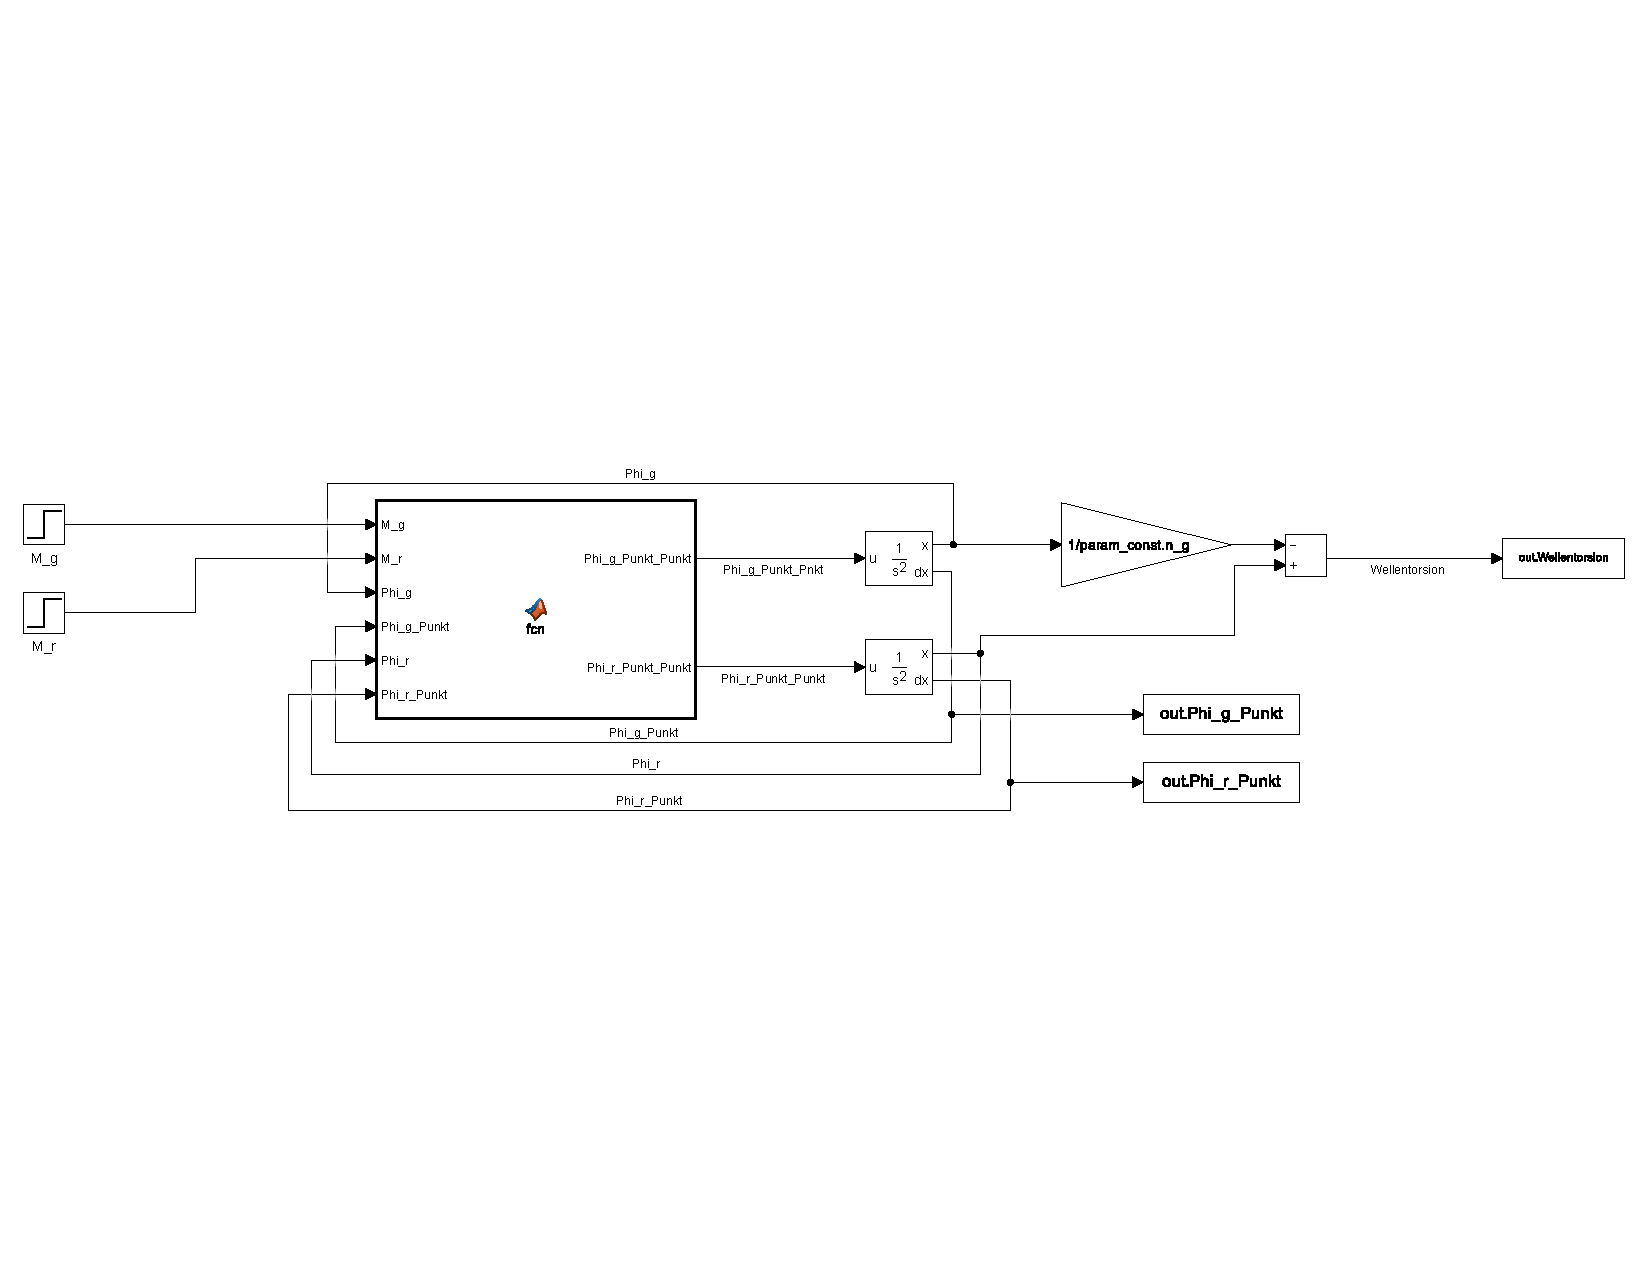
\includegraphics[width=1.0\textwidth]{Bilder/Kapitel 4/Blockstruktur_Antriebsstrang.pdf}}
   \caption[Antriebsstrang Simulink]{Simulink Blockstruktur des Antriebsstranges der WEA}
   \label{fig:Bild3.3}
\end{figure}

\autoref{fig:Bild3.3} zeigt die Blockstruktur, welche in Simulink umgesetzt wurde. Der Funktionsblock in der Mitte der Abbildung enthält die Modellgleichungen, welche zuvor in \autoref{eq:Gleichung3.9} und \autoref{eq:Gleichung3.10} hergeleitet wurden. Eingangsseitig wird ein Sprung von \acs{MG} \bzw \acs{MR} eingeprägt. Ersterer setzt nach \SI{15}{s} ein, Zweiterer bereits nach \SI{5}{s}. Ausgangsseitig werden durch die Nutzung von Integratoren die Winkelgeschwindigkeiten \acs{omegaR} und \acs{omegaG} zurückgegeben. Für die Modellverifikation wurde noch ein weiterer Ausgang hinzugefügt, welcher die Differenz des \ac{phiR} und des \ac{phiG} bereitstellt. \\

In \autoref{fig:Bild3.4} ist klar zu erkennen, dass durch die Einprägung des Momentensprunges auf den Rotor die Winkelgeschwindigkeit der Welle annähernd linear ansteigt. Dies zeigt sich sowohl auf Seiten des Rotors als auch auf Seiten des Generators. Der Kurvenverlauf beider Winkelgeschwindigkeiten ist annähernd identisch. Der Unterschied um zwei Zehnerpotenzen ergibt sich aus der \acf{ng}, welche bei \ca 100 (97) liegt.\\
Der generatorseitige Momentensprung zeigt sich in \autoref{fig:Bild3.4} besonders gut in der Betrachtung der \ac{dotphiG}. Es kommt zu einem Schwingvorgang, der nach etwas über \SI{5}{s} wieder ausgeglichen ist. Durch die Elastizität der Welle ist der Momentensprung am Generator rotorseitig abgedämpft. Die \ac{dotphiR} schwingt nur leicht.

\begin{figure}[H]
   \centering
   \fbox{\includegraphics[width=0.76\textwidth]{Bilder/Kapitel 4/Winkelgeschwindigkeiten.pdf}}
   \caption[Winkelgeschwindigkeiten Antriebsstrang]{Visualisierung der Winkelgeschwindigkeit des Rotors und des Generators nach zeitversetzter Sprunganregung}
   \label{fig:Bild3.4}
\end{figure}

\autoref{fig:Bild3.5} zeigt die Differenz zwischen Rotorwinkel (\acs{phiR}) und Generatorwinkel (\ac{phiG}). Diese gibt eine Aussage darüber, inwiefern es zu einer Torsion der Antriebswelle kommt. Es ist zu erkennen, dass nach \SI{5}{s} eine erste Torsion auftritt, die sich nach kurzem Schwingen auf einen stationären Wert von rund einem Millionstel eines Grades einpegelt. Nach dem generatorseitigen Momentensprung (bei \SI{15}{s} kommt es erneut zu einem Schwingvorgang in der Wellentorsion. Da das eingeprägte Moment signifikant größer ist, ist die Schwingungsamplitude ebenfalls deutlich größer als zuvor beim rotorseitigen Momentensprung. Nach \ca \SI{10}{s} ist auch dieser Schwingvorgang abgeschlossen und ein stationärer Endwert von rund einem Einhunderttausendstel Grad wird erreicht. \\
Es kann zusammenfassend argumentiert werden, dass die Simulationsergebnisse plausibel und hinreichend genau sind, um das Antriebsstrangmodell als Teilmodell der Simulation und Regelung der Windenergieanlage einsetzen zu können.

\begin{figure}[H]
   \centering
   \fbox{\includegraphics[width=0.76\textwidth]{Bilder/Kapitel 4/Wellentorsion.pdf}}
   \caption[Wellentorsion Antriebsstrang]{Visualisierung der Wellentorsion des Antriebsstranges nach zeitversetzter Sprunganregung}
   \label{fig:Bild3.5}
\end{figure}